\chapter{Introduction}

\section{Research background}

Machine learning tries to answer the question of how could computers be trained to do useful work without having been explicitly programmed to do so. Machine learning subject area can be divided into many subcategories, and neural networks are one of them. Neural networks are constructed from simple functions which are composed together to form networks. The functional parts of neural networks are inspired by neuroscience, which is the scientific study of nervous systems. Neural networks have been shown to be able to solve many different and difficult problems, especially in the area of computer vision. \cite{Goodfellow2016,LeCun2015}

Research about automated face detection, i.e., determining if an image contains a face or not, dates back to the beginning of the 1970s \cite{Sakai1972}. Since then the methods have been improved so that real-time detection of multiple faces from an image or video is possible \cite{Osadchy2007}. In contrast to face detection, face reconstruction strives to extract the underlying 3D model of the facial geometry. It can be done today accurately but usually needs multiple images of the face \cite{Valgaerts2012}. Face recognition methods try to detect if a specific person is in the image. Face recognition methods analyze human faces on a deeper level than face detection methods, but the recognition methods do not need to process as much facial detail as the reconstructions methods \cite{Datta2015}. Automated single image facial geometry reconstruction is still an active area of research.

In recent years, the capabilities of machine learning methods have greatly increased, and this new era of machine learning has been named ''deep learning`` \cite{Goodfellow2016}. What is new is the massively increased computing power and memory capacity of the newer \acp{GPU} and the lucky fact that the neural network training and inference map very well to \ac{GPU} hardware architectures. Coupled with small algorithmic tweaks \cite{Goodfellow2016}, this has allowed successful training of very deep neural networks with tens of millions of parameters, hence the name deep learning. Deep networks are beneficial because they can automatically learn, from large amounts of raw data, the representations needed for the task at hand \cite{LeCun2015}. Also, numerous Python-based \ac{GPU}-accelerated deep learning frameworks have emerged in the last few years which allow rapid implementation and iteration of the network models \cite{tensorflow,cntk}.

\acp{CNN} have been used for image processing since the late 1980s \cite{LeCun1989}. Lately, they have been increasingly used in, for example, face detection \cite{Osadchy2007} and face reconstruction \cite{Richardson2016a}. \acp{CNN} have been shown to be able to extract low dimensional representations of facial pose and appearance parameters which could consequently be used for reconstructing the facial geometry \cite{Kim2017}. Very recently, the \acp{CNN} have been extended to \acp{FCNN} that could do semantic segmentation, i.e., dense pixel-to-pixel mapping \cite{Long2015,Isola2016}. In other words, \acp{FCNN} can take in an image, process it, and output another image.

Training of the deep neural networks in a supervised manner, i.e., with input/output pairs of known data, needs a large amount of annotated material. Training the networks to do face detection is relatively easy because the data annotations are light-weight and easily generated manually \cite{Osadchy2007}. To train the networks to do facial reconstruction is considerably harder because the training data needs to be densely annotated, and the annotations are almost impossible to create by hand \cite{Richardson2016a}. It is possible though to produce human face images and their dense geometry annotations using computer graphics. The obvious problem, in this case, is that the synthetic face images cannot be completely realistic. Instead of trying to generate as realistic face images as possible, it might be possible to go all the way to the other direction and generate a vast number of completely unrealistic facial images with greatly varying colors and textures. This way the only thing that is not randomized is the basic principles of light interaction with the geometry of the face. The network would have to learn to ignore everything else. \textcite{Tobin2017} proposed an idea called domain randomization in the context of robot machine vision and simple scenes of various objects. They trained their vision neural network using greatly varying non-realistic renders of the scene and got the network to generalize to real-world. They argued that because of enough variation in the training data, the neural network learned to see the reality as just another variation. This thesis has a similar idea, but we came up with it independently.

Abundant processing power and storage capacity is nowadays available in computing clusters, and it is feasible to generate large sets of densely annotated training images by rendering \cite{Movshovitz-Attias2016}. Modern 3D modelers/renderers like \textcite{blender} have the ability to output realistic images, be completely scripted, and be run from the command line in computing clusters \cite{blender}. In addition, it has been shown that the effective sizes of training datasets can be increased by, for example, randomly swapping the color channels of the training images \cite{Wu2015}. This is called data augmentation \cite{Goodfellow2016}. Generalization in machine learning means that the trained network works well on input it has not seen in the training data. Overfitting means the network has learned the training data well but does not generalize well to unseen input. Data augmentation makes it possible to use smaller datasets while preventing the network from overfitting and getting it to generalize well to new data \cite{Goodfellow2016}.

\section{Research problem}

\begin{figure}
    \centering
    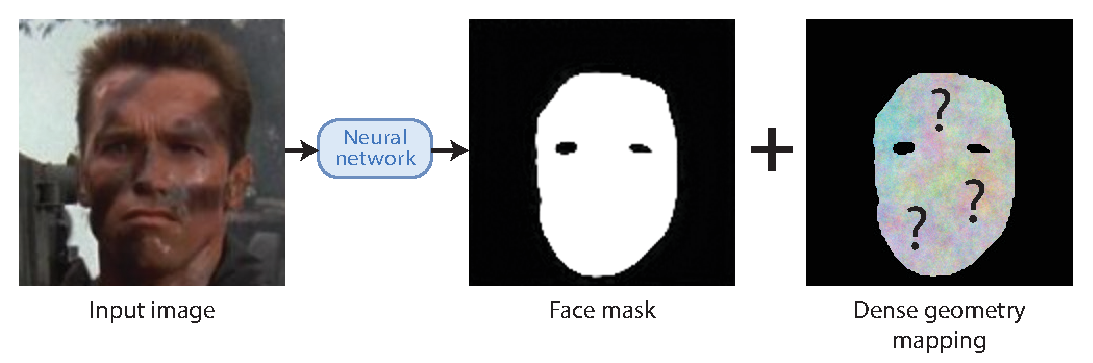
\includegraphics[width=\textwidth]{problem}
    \caption[Main research goal]{The main research goal visualized. A \acf{FCNN} is given a real-world human face image as an input, and the result should be the face segmented out of the background and densely filled with useful geometry information.}
    \label{fig:research_problem_1}
\end{figure}

\acp{CNN} have been shown to be able to extract relevant information from human faces, and the extension of \acp{CNN}, \acp{FCNN}, has been shown to be able to do dense pixel-to-pixel mappings in various situations. Could it be possible to train an \ac{FCNN} to extract human facial geometry information from an image and map it to another presentation densely pixel-per-pixel (see figure \ref{fig:research_problem_1})? An \ac{FCNN} can be trained in a supervised manner using a large number of densely annotated image pairs, but those are not readily available for real-world human faces. Could it be possible to generate these training pairs by rendering? Could the rendered data be non-realistic and still make it possible for the trained \ac{FCNN} to generalize to real-world images? What is the mapping that could be generated by rendering and that is possible for the \ac{FCNN} to learn? Could the rendered training dataset be extended using data augmentation to prevent overfitting and to enable occlusion detection?

\section{Research goals}

The main research goal of this thesis is to train a \acf{FCNN} using non-realistic synthetic data to do dense human facial geometry tracking on real-world images. If the network is given an image of a real human face as an input, the output should be a same sized image with the face segmented out of the background and filled with a useful dense geometry mapping. The main research goal is visualized in figure \ref{fig:research_problem_1}.

\newpage

This main goal can be divided into seven subgoals:

\begin{itemize}
    \item Design and implement a suitable network topology and a loss function using a Python-based deep learning framework, e.g., \textcite{cntk}. If the topology and loss functions are good enough, the network should produce non-blurry, sharply defined, results with a reasonable number of parameters.
    \item Design and implement a method to generate a large quantity of non-realistic synthetic training data in a reasonable amount of time. The dataset should be big enough and have a precise enough mapping that the training of the \ac{FCNN} is possible. Also, rendering a new dataset should take less than 24 hours.
    \item Make the network generalize well to real-world images of human faces. Even if the network is trained on completely non-realistic data, the network should be able to detect real-world faces and extract relevant geometry information from them.
    \item Make the feature detection of the network invariant to lighting, texturing, scaling and positioning. Even if the subject in the real-world image is under extreme conditions, the network should continue to output believable segmentation and geometry mapping.
    \item Enable the network to inpaint believable geometry under occlusions. If the face is, for example, partially occluded by sunglasses, the network should be able to detect them and generate geometry underneath.
    \item Implement geometry mapping visualizations and, in general, make the evaluation of results easy. It should be possible to see how well the generated geometry matches the real subject, and comparing results between different network versions should be effortless.
    \item Make the network generate temporally stable geometry mappings when applied to video. When looking at a video, the generated geometry should not flicker and jump around from frame to frame.
\end{itemize}

\section{Research scope}

The scope of this thesis includes the neural network design, synthetic data generation, data augmentation, training of the network, geometry mapping visualizations, and evaluation of the results. The facial geometry is identified in the canonical 2D parameterization. Because of time constraints, the extraction of 3D geometry from the parameterization has not been included.

